%!TEX root = Python.tex

\chapter{Entrada y salida}

\lettrine[lines=5]{P}{ara} realizar aplicaciones medianamente útiles con Python tenemos que estudiar algunas herramientas más del lenguaje relativas a la entrada y salida de información de las aplicaciones. En este capítulo comenzamos viendo el modo de consultar los argumentos de un programa Python. A continuación comentaremos el uso de la entrada estándar, salida estándar y salida de errores. Para lograr cierta persistencia en los datos necesitaremos también almacenar y recuperar información de ficheros. Por esta razón, completaremos este capítulo con una explicación de la funcionalidad que ofrece Python para manejar el acceso a ficheros.

\section{Argumentos del programa}

Supongamos que queremos desarrollar una aplicación con Python que se va a ejecutar desde la consola del sistema operativo. Este tipo de aplicaciones suelen recibir información en forma de argumentos de la línea de comandos. Por ejemplo, si la aplicación está implementada en un módulo llamado \texttt{a.py} y recibe tres argumentos, se podría lanzar así:

\begin{lstlisting}
$ python a.py arg1 arg2 arg3
\end{lstlisting}

El intérprete de Python coloca los argumentos con los que se ha invocado a la aplicación en la lista \texttt{sys.argv}. 

\begin{lstlisting}
import sys

if __name__ == '__main__':
    if len(sys.argv) != 4:
        print('Uso: %s arg1 arg2 arg3' % (sys.argv[0]))
    else:
        arg1 = sys.argv[1]
        arg2 = sys.argv[2]
        arg3 = sys.argv[3]
\end{lstlisting}

Al igual que sucede con los programas en C, el argumento \texttt{sys.argv[0]} contiene el nombre del script. Para indicar los argumentos desde Eclipse, tenemos que entrar en las propiedades del módulo \texttt{a.py} en el explorador de archivos (botón derecho del ratón sobre el fichero) y a continuación editamos \emph{Run/Debug Settings}. Veremos un formulario como el mostrado en la figura \ref{fig:argumentos} con una solapa \emph{arguments} en la que podemos introducir los argumentos.

\begin{figure}
\begin{center}
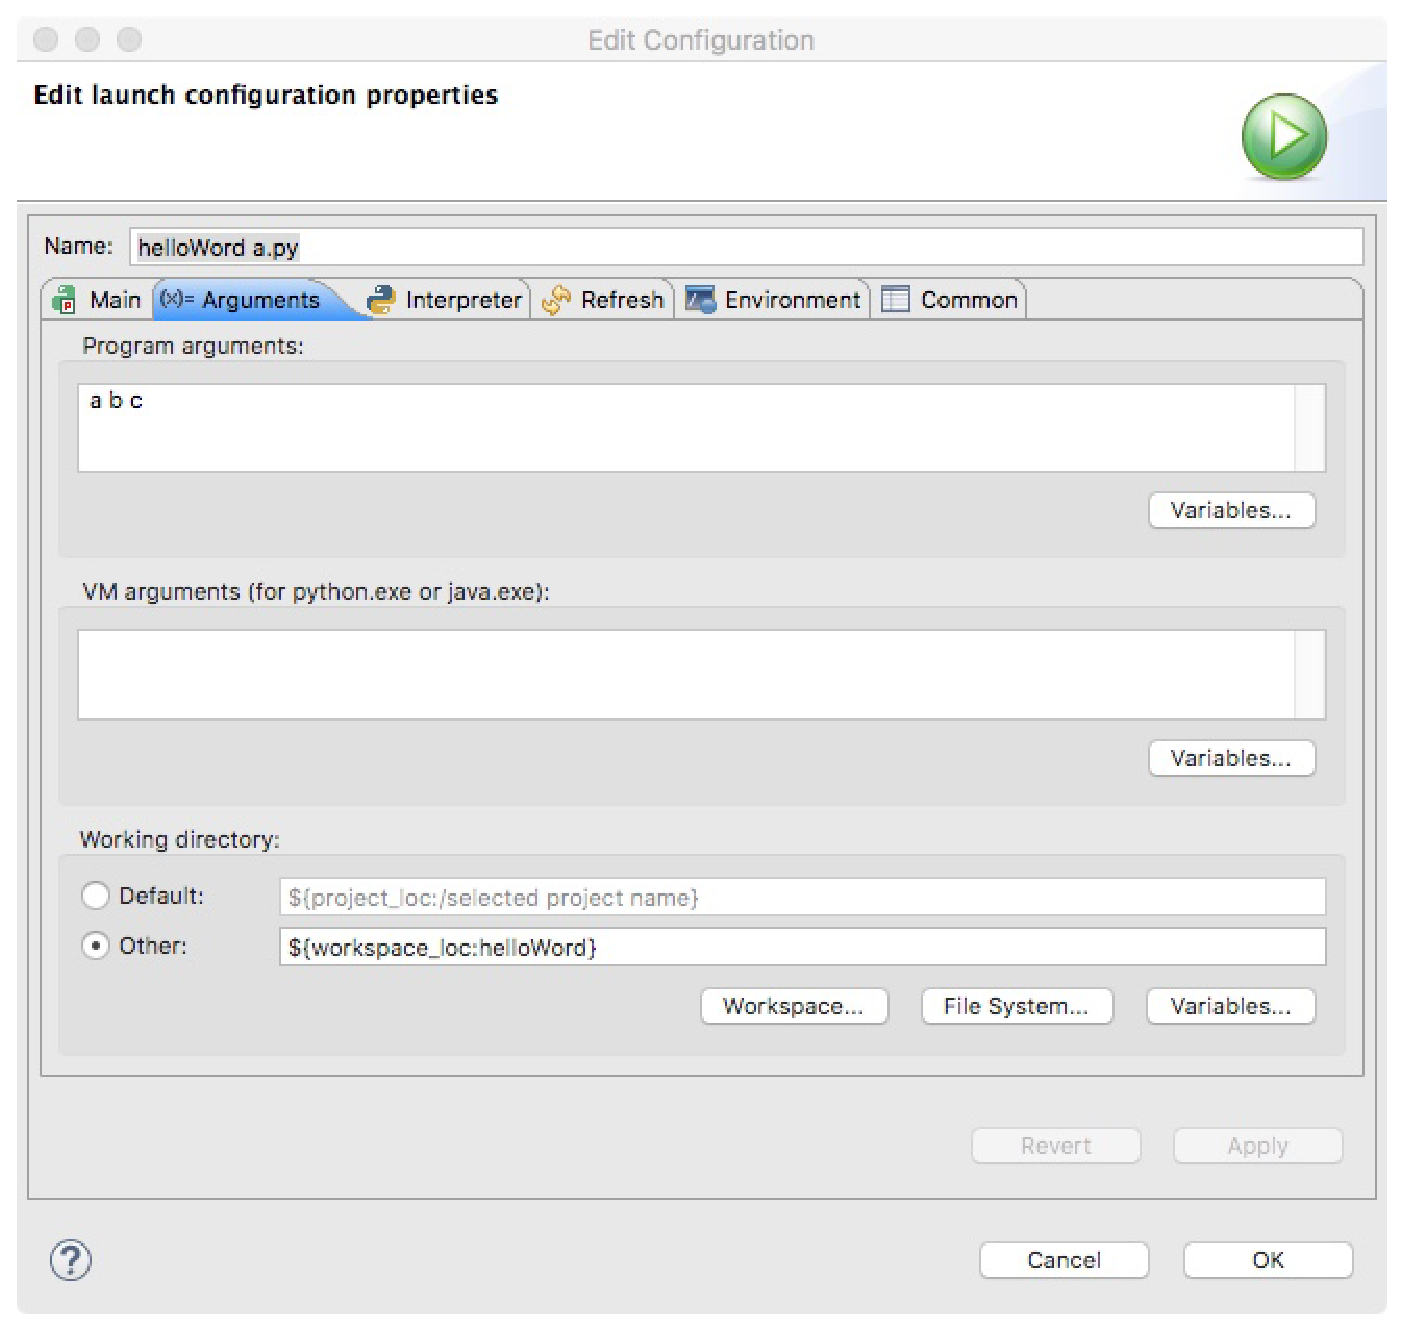
\includegraphics[height=0.65\textwidth]{imagenes/arguments}
\end{center}
\caption{Configuración de argumentos en Eclipse}
\label{fig:argumentos}
\end{figure}

\section{Entrada, salida y errores}

El módulo \texttt{sys}, que hemos usado en el apartado anterior para consultar los argumentos del programa, también nos ofrece tres \emph{flujos} (streams) abiertos para manejar la entrada estándar al programa, la salida estándar y la salida de errores. Se trata de \texttt{sys.stdin}, \texttt{sys.stdout} y \texttt{sys.stderr}. 

Aunque es posible manejar estos flujos de entrada y salida directamente usando las herramientas de lectura y escritura de archivos, en esta sección comentamos el modo de emplearlos indirectamente a través de los métodos \texttt{input()} y \texttt{print()}.

\subsection{Entrada estándar}

El modo más sencillo para leer de la entrada estándar es la función \texttt{input()}, incluida en el propio lenguaje. La función lee una línea completa de la entrada, la convierte a una cadena (eliminando el salto de línea) y la devuelve. Opcionalmente podemos llamar a \texttt{input()} con un argumento que es el \emph{promt} que se mostrará al usuario por salida estándar para invitarle a que escriba:

\begin{lstlisting}
print("Indica tu sketch de los Monty Python favorito")
sketch = input("--> ")
best = ['The Spanish Inquisition','Four Yorkshiremen','Brain Specialist']
if sketch in best:
	print("¡Ése es genial!")
else:
    print("No está mal")
\end{lstlisting}

\subsection{Salida estándar y salida de errores}

Ya hemos visto el uso del método \texttt{print()} en bastantes ejemplos, pero podría indicarse algo más. Hasta ahora, hemos usado \texttt{print()} con uno o varios argumentos separados por comas, y el comportamiento que tiene por defecto consiste en imprimir las cadenas que resultan de invocar a \texttt{str()} sobre cada argumento, dejando un espacio en blanco como separador. Podemos modificar el separador usando el argumento nombrado \texttt{sep}:

\begin{lstlisting}
print('Uno',2,['a','b',3],sep='.+.')
\end{lstlisting}

Un segundo argumento adicional del método \texttt{print()} es \texttt{file}, que permite especificar el flujo a través del cual se va a generar la salida. Por defecto toma el valor \texttt{sys.stdout}, pero podemos usarlo para producir mensajes de error a través de \texttt{sys.stderr}:

\begin{lstlisting}
print('¡Catástrofe: excepción capturada!',file=sys.stderr)
\end{lstlisting}

Los mensajes enviados a la salida de error se muestran en rojo en la consola de Eclipse. Dependiendo del funcionamiento del intérprete de Python, los mensajes de la salida estándar y la salida de error se pueden mezclar. Esto se debe a que los accesos a la consola se intentan reducir para acelerar la ejecución del programa. El texto pendiente de ser emitido por la consola se almacena en un buffer que, llegado el momento que decida el intérprete, se muestra por la salida. Si sólo se usa una salida (normal o de error), no hay problema en la ordenación de los mensajes. Si se emplean las dos, podemos encontrarnos con mezclas extrañas. Para obligar a que se vacíe un flujo en la consola, el método \texttt{print()} tiene otro argumento más: \texttt{flush}. Por defecto toma el valor \texttt{False}, indicando que no hay que imprimir inmediatamente la salida. Si se indica \texttt{True} se fuerza al intérprete a emitir por consola todo lo que tenga almacenado en el buffer asociado al flujo del argumento \texttt{file}.

Otro argumento que puedes usar con el método \texttt{print()} es \texttt{end}. Por defecto, el método genera un salto de línea como último caracter de la cadena que se imprime. Podemos modificar este comportamiento especificando otra cadena en \texttt{end}:

\begin{lstlisting}
print('No imprimas un salto ',end='')
print('porque quiero seguir en la misma línea')
\end{lstlisting}


\section{Ficheros}

Python incluye una función integrada en el propio lenguaje para abrir archivos del sistema: \texttt{open()}. El resultado de la función es una instancia de un tipo de dato que actúa como \emph{descriptor de archivo} y que ya hemos usado con los flujos de entrada estándar, salida estándar y error. Sobre los descriptores de archivo abiertos podremos invocar a una serie de métodos para realizar operaciones de lectura, escritura y cierre de los archivos.

\subsection{Apertura}

El uso más básico del método \texttt{open()} consiste en proporcionarle como argumento el nombre del archivo que queremos abrir. El nombre puede incluir una ruta de directorios delante. Si no la tiene, Python considera que está en el mismo directorio en el que se encuentra el módulo que realiza la apertura. Para usuarios de Windows es importante tener en cuenta que las rutas de archivos usan la contrabarra como separador de directorios. Por esta razón, será conveniente usar el prefijo \texttt{r} en la cadena, de modo que la contrabarra no se interprete como parte de un carácter de escape.

\begin{lstlisting}
archivo = open(r'C:\spam.txt')	
\end{lstlisting}

Por defecto, el modo de apertura es para \emph{lectura}. Y sí, lo has adivinado: si el archivo no existe, excepción al canto. En este caso sería de tipo \texttt{FileNotFoundError}. Por tanto, si no te gusta el riesgo, pon un buen \texttt{try-except} rodeando la apertura del archivo.

Para indicar el modo de apertura, ya sea lectura o escritura, se puede pasar un segundo argumento al método \texttt{open} en forma de cadena de caracteres que tiene el significado siguiente:
\begin{itemize}
	\item \texttt{r}: apertura en modo lectura, que es el modo por defecto. Se lee el fichero desde el comienzo.
	\item \texttt{w}: apertura en modo escritura. Si el fichero existe, lo vacía.
	\item \texttt{a}: apertura en modo escritura. Si el fichero existe, no lo vacía sino que añade lo que se escriba al final del mismo.
	\item \texttt{x}: apertura en modo escritura. Si el fichero existe, salta una excepción \texttt{FileExistsError}.
\end{itemize}

Para abrir un fichero en modo lectura y escritura simultáneamente, hay que añadir el carácter \texttt{+} al modo de apertura. Normalmente se empleará la operación \texttt{seek()} que luego se describe para situar la posición de la seguiente operación de lectura o escritura:
\begin{itemize}
	\item \texttt{r+}: apertura en modo lectura y escritura sin vaciar el fichero. Inicialmente se escribe y lee por el principio.
	\item \texttt{w+}: apertura en modo lectura y escritura, vaciando el fichero si existe.
	\item \texttt{a+}: apertura en modo lectura y escritura. Si el fichero existe, inicialmente se escribe y lee al final del mismo.
	\item \texttt{x+}: apertura en modo lectura y escritura. Si el fichero existe, salta una excepción de tipo \texttt{FileExistsError}.
\end{itemize}

Detras de la indicación del modo de apertura, en la misma cadena, se puede indicar si se quiere manejar el fichero en modo texto o binario:
\begin{itemize}
	\item \texttt{t}: apertura en modo texto, que es el modo por defecto.
	\item \texttt{b}: apertura en modo binario.
\end{itemize}

\begin{lstlisting}
# Apertura en modo lectura/escritura para texto
archivo = open('log.txt','r+t')
\end{lstlisting}

El argumento con el modo de apertura tiene que indicarse en segundo lugar, o bien puede nombrarse con \texttt{mode=}. Un argumento que se nombra con \texttt{encoding} permite especificar cuál es el código de caracteres con el que se debe tratar el archivo. Si no se indica, se manejará el código de caracteres del sistema. Por ejemplo, en Windows se emplea \texttt{cp1252} (una extensión de \texttt{latin1}), pero otros sistemas como Mac OS X o Linux usan \texttt{utf8}:

\begin{lstlisting}
# Apertura en modo escritura con latin1
archivo = open('salida.txt','w',encoding='latin1')
\end{lstlisting}

\subsection{Lectura}

Existen varias posibilidades al leer un archivo con Python: leerlo completamente en una única operación, leerlo línea a línea o leerlo en fragmentos de cierta cantidad de bytes. Vemos por separado cada alternativa.

\subsubsection{Lectura completa}

El modo más sencillo para leer un archivo consiste en invocar al método \texttt{read()} sobre el mismo una única vez:

\begin{lstlisting}
archivo = open('archivo.txt')
contenido = archivo.read()
\end{lstlisting}

En la variable \texttt{contenido} se queda almacenada una cadena con todo el contenido del archivo. Sobre esta cadena se pueden usar los métodos de indexación, troceado o fragmentación que sean necesarios para procesar el contenido.

\subsubsection{Lectura por líneas}

En muchas ocasiones, el procesamiento de un archivo se debe realizar línea a línea. Python nos da tres alternativas para leer una tras otra todas las líneas de un archivo: el método \texttt{readline()} que se invoca sobre el archivo abierto, un iterador sobre el archivo, o bien el método \texttt{readlines()}, que devuelve una lista con todas las líneas del archivo.

El método \texttt{readline()} devuelve sucesivamente las líneas del fichero abierto, incluyendo el salto de línea. Cuando no quedan más líneas, el método devuelve la cadena vacía:

\begin{lstlisting}
archivo = open(nombre)
n = 1
while True:
    línea = archivo.readline()
    if not línea:
        break # Final del archivo
    else:
        print('Línea %d: -%s-' % (n,línea.rstrip()))
        n += 1
\end{lstlisting}

Recuerda que la estructura del \texttt{while} anterior, sólo apta para estómagos fuertes, es una forma de escribir un \emph{do-while} en Python. Una alternativa más elegante para hacer lo mismo consiste en usar un \texttt{for-in} sobre el archivo abierto, que en Python es un objeto sobre el que se puede implementar una iteración:

\begin{lstlisting}
archivo = open(nombre)
n = 1
for línea in archivo:
    print('Línea %d: -%s-' % (n,línea.rstrip()))
    n += 1
\end{lstlisting}

Y vamos con la tercera alternativa: el método \texttt{readlines()}. Mediante este método podemos obtener todas las líneas del archivo en una lista:

\begin{lstlisting}
archivo = open(nombre)
líneas = archivo.readlines()
n = 1
for línea in líneas:
    print('Línea %d: -%s-' % (n,línea.rstrip()))
    n += 1
\end{lstlisting}

Es cuestión de gustos el escoger una u otra.

\subsubsection{Lectura por caracteres o bytes}

Una posibilidad más a la hora de leer los archivos -- especialmente útil cuando se trata de archivos binarios -- es la lectura de bloques de bytes o caracteres. Para ello tenemos que emplear una versión de \texttt{read()} que tiene como argumento el número de bytes o caracteres que se quiere leer:

\begin{lstlisting}
tamaño_cabecera = 10
archivo = open(nombre,"rb")
cabecera = archivo.read(tamaño_cabecera)
for b in cabecera:
	print('%x' % (b), end=' ')
\end{lstlisting}


\subsection{Escritura}

Lo sentimos por los programadores indecisos: también tenemos varias formas de escribir en un fichero. Podemos emplear los métodos \texttt{write()} y \texttt{writelines()} del fichero abierto en modo escritura, o bien podemos usar \texttt{print()} especificando en el parámetro \texttt{file} el fichero.

El método \texttt{write()} es el clásico. Tiene como argumento la cadena que se quiere imprimir, que es una cadena de caracteres en caso de que se haya abierto en modo texto, o bien una cadena binaria si se ha abierto en modo binario:

\begin{lstlisting}
archivo = open('salida.txt','w',encoding='latin1')
archivo.write('De minimis non curat praetor\n')
archivo.write('Aquila non capit muscas\n')
archivo.write('Beati hispani quibus vivere bibere est\n')
\end{lstlisting}

Como alternativa, en caso de que tengamos una lista de cadenas y queramos volcarlas sobre el archivo en el orden en el que se encuentran en la lista, podemos emplear \texttt{writelines()}:

\begin{lstlisting}
archivo = open('salida.txt','w',encoding='latin1')
latinajos = []
latinajos += ['De minimis non curat praetor\n']
latinajos += ['Aquila non capit muscas\n']
latinajos += ['Beati hispani quibus vivere bibere est\n']
archivo.writelines(latinajos)
\end{lstlisting}

Y como tercera alternativa, tenemos el método \texttt{print()} con el argumento \texttt{file}:

\begin{lstlisting}
archivo = open('salida.txt','w')
print('%.2f*%.2f+%.2f=%.2f' % (3.14,2.0,5.1,3.14*2.0+5.1), file=archivo)
\end{lstlisting}

\subsection{Otros métodos}

Para concluir la descripción de las operaciones sobre archivos, comentamos brevemente tres métodos más. En primer lugar, el método de cierre: \texttt{close()}. Como hemos indicado en varias ocasiones, Python emplea un \emph{recolector de basura} para liberar la memoria que ya no se referencia en nuestro programa. Esta recolección incluye a los ficheros abiertos que ya no se pueden usar porque el código ha pasado a otro ámbito y no son alcanzables. Python cierra automáticamente estos archivos antes de liberar los recursos que emplean. Pero nosotros podemos realizar el cierre de forma explícita:

\begin{lstlisting}
archivo.close()
\end{lstlisting}

El cierre lleva a cabo un vaciado del buffer de salida que el intérprete de Python puede estar usando para reducir el acceso al disco. También podemos forzar ese vaciado sin cerrar el archivo, invocando al método \texttt{flush()}:

\begin{lstlisting}
archivo.flush()
\end{lstlisting}

Por último, cuando un archivo se abre en modo lectura y escritura (incluyendo \texttt{+} en el modo de apertura), es muy posible que necesitemos situarnos en diferentes posiciones del archivo en función de la operación que queramos hacer. Sabiendo el desplazamiento \texttt{N} desde el comienzo del fichero, podemos indicar la posición de la siguiente lectura o escritura usando \texttt{seek()}:

\begin{lstlisting}
archivo.seek(N)
\end{lstlisting}

